\section{Design patterns}
Tijdens het realiseren van de afstudeer opdracht is er gebruik gemaakt van het Repository pattern.
Dit pattern en een \textbf{ander pattern wat ik nog moet verzinnen} zijn beschreven in de volgende delen.

\subsection{Repository pattern}
Het repository pattern is een structureel design pattern dat de datalaag en logica van de applicatie scheidt.
Dit wordt bereikt door middel van een abstracte tussenlaag die communicatie mogelijk maakt tussen de logica en de datalaag.

\whitespace
Dit leidt tot een scheiding tussen de logica en de data, waardoor voldaan wordt aan het Single Responsibility Principle.
Dit resulteert in beter testbare code, wat de betrouwbaarheid van het programma verhoogt.
Bovendien voorkomt dit dat de codebase afhankelijk is van één specifieke databaseprovider.

\whitespace
Dit is geimplementeerd door de logica af te laten hangen van een interface inplaats van een concrete implementatie.
Vervolgens wordt bij initialisatie van de applicatie  een concrete versie \textit{gedependency inject}.
Een visualisatie van de geïmplementeerde versie is te zien in figuur \ref{fig:RepositoryPattern}

\whitespace[2]
\begin{graphic}
    \captionsetup{type=figure}
    \caption{Visualisatie van fields}
    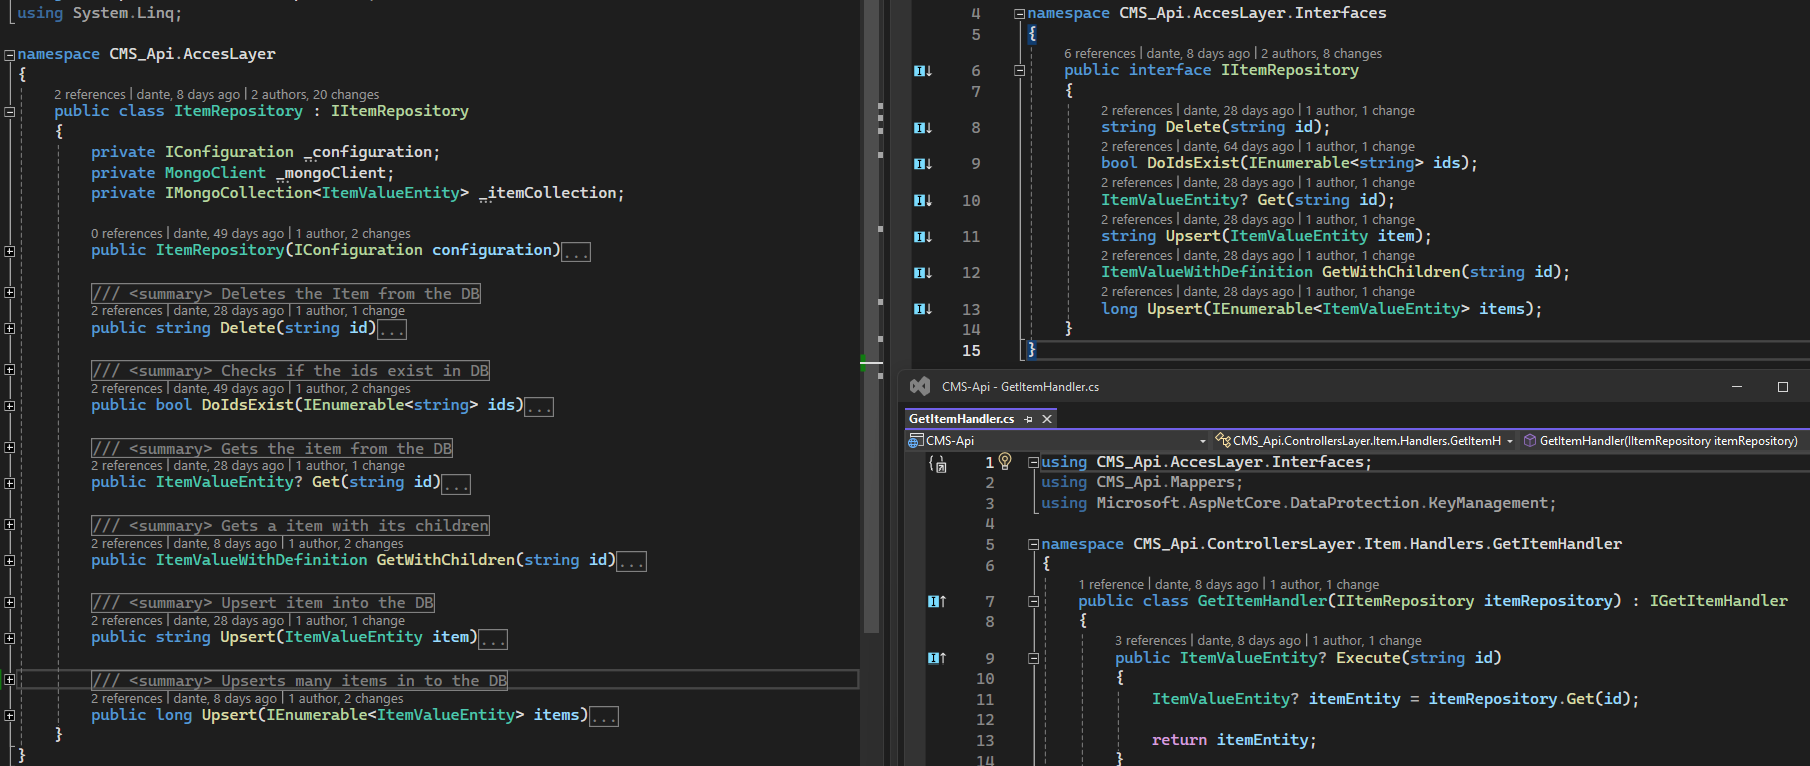
\includegraphics[scale=0.35]{ImplementationRepositoryPattern.png}
    \label{fig:RepositoryPattern}
\end{graphic}
% Het repository pattern is een structural design pattern dat gebruikt wordt om je logica en data \textit{retrieval} te scheiden.
% Door de datalaag te schieden van de logica moet het makkelijker worden om nieuwe databases of andere data storage methodes te implementeren.

\subsection{Flightweight pattern}
yes mabey
